
%% bare_conf.tex
%% V1.3
%% 2007/01/11
%% by Michael Shell
%% See:
%% http://www.michaelshell.org/
%% for current contact information.
%%
%% This is a skeleton file demonstrating the use of IEEEtran.cls
%% (requires IEEEtran.cls version 1.7 or later) with an IEEE conference paper.
%%
%% Support sites:
%% http://www.michaelshell.org/tex/ieeetran/
%% http://www.ctan.org/tex-archive/macros/latex/contrib/IEEEtran/
%% and
%% http://www.ieee.org/

%%*************************************************************************
%% Legal Notice:
%% This code is offered as-is without any warranty either expressed or
%% implied; without even the implied warranty of MERCHANTABILITY or
%% FITNESS FOR A PARTICULAR PURPOSE! 
%% User assumes all risk.
%% In no event shall IEEE or any contributor to this code be liable for
%% any damages or losses, including, but not limited to, incidental,
%% consequential, or any other damages, resulting from the use or misuse
%% of any information contained here.
%%
%% All comments are the opinions of their respective authors and are not
%% necessarily endorsed by the IEEE.
%%
%% This work is distributed under the LaTeX Project Public License (LPPL)
%% ( http://www.latex-project.org/ ) version 1.3, and may be freely used,
%% distributed and modified. A copy of the LPPL, version 1.3, is included
%% in the base LaTeX documentation of all distributions of LaTeX released
%% 2003/12/01 or later.
%% Retain all contribution notices and credits.
%% ** Modified files should be clearly indicated as such, including  **
%% ** renaming them and changing author support contact information. **
%%
%% File list of work: IEEEtran.cls, IEEEtran_HOWTO.pdf, bare_adv.tex,
%%                    bare_conf.tex, bare_jrnl.tex, bare_jrnl_compsoc.tex
%%*************************************************************************

% *** Authors should verify (and, if needed, correct) their LaTeX system  ***
% *** with the testflow diagnostic prior to trusting their LaTeX platform ***
% *** with production work. IEEE's font choices can trigger bugs that do  ***
% *** not appear when using other class files.                            ***
% The testflow support page is at:
% http://www.michaelshell.org/tex/testflow/



% Note that the a4paper option is mainly intended so that authors in
% countries using A4 can easily print to A4 and see how their papers will
% look in print - the typesetting of the document will not typically be
% affected with changes in paper size (but the bottom and side margins will).
% Use the testflow package mentioned above to verify correct handling of
% both paper sizes by the user's LaTeX system.
%
% Also note that the "draftcls" or "draftclsnofoot", not "draft", option
% should be used if it is desired that the figures are to be displayed in
% draft mode.
%
\documentclass[10pt, conference, compsocconf]{IEEEtran}
% Add the compsocconf option for Computer Society conferences.
%
% If IEEEtran.cls has not been installed into the LaTeX system files,
% manually specify the path to it like:
% \documentclass[conference]{../sty/IEEEtran}



\usepackage{color}
\usepackage{graphicx}
\usepackage{listings}

\lstset{language=C,
        frame=none,%single,
        basicstyle=\ttfamily,
        keywordstyle=\bfseries,
        commentstyle=\em,
        tabsize=2,
        showstringspaces=false,
        flexiblecolumns=false,
        mathescape=true,
        escapeinside={\#}{\#},
        % numbers=left, numberstyle=\tiny, numbersep=5pt %, stepnumber=2, 
        numbersep=5pt,
        % literate={->}{{$\rightarrow$}}1 {<->}{{$\leftarrow$}}1
}
\newcommand\x[1]{\lstinline{#1}}


% Some very useful LaTeX packages include:
% (uncomment the ones you want to load)


% *** MISC UTILITY PACKAGES ***
%
%\usepackage{ifpdf}
% Heiko Oberdiek's ifpdf.sty is very useful if you need conditional
% compilation based on whether the output is pdf or dvi.
% usage:
% \ifpdf
%   % pdf code
% \else
%   % dvi code
% \fi
% The latest version of ifpdf.sty can be obtained from:
% http://www.ctan.org/tex-archive/macros/latex/contrib/oberdiek/
% Also, note that IEEEtran.cls V1.7 and later provides a builtin
% \ifCLASSINFOpdf conditional that works the same way.
% When switching from latex to pdflatex and vice-versa, the compiler may
% have to be run twice to clear warning/error messages.






% *** CITATION PACKAGES ***
%
%\usepackage{cite}
% cite.sty was written by Donald Arseneau
% V1.6 and later of IEEEtran pre-defines the format of the cite.sty package
% \cite{} output to follow that of IEEE. Loading the cite package will
% result in citation numbers being automatically sorted and properly
% "compressed/ranged". e.g., [1], [9], [2], [7], [5], [6] without using
% cite.sty will become [1], [2], [5]--[7], [9] using cite.sty. cite.sty's
% \cite will automatically add leading space, if needed. Use cite.sty's
% noadjust option (cite.sty V3.8 and later) if you want to turn this off.
% cite.sty is already installed on most LaTeX systems. Be sure and use
% version 4.0 (2003-05-27) and later if using hyperref.sty. cite.sty does
% not currently provide for hyperlinked citations.
% The latest version can be obtained at:
% http://www.ctan.org/tex-archive/macros/latex/contrib/cite/
% The documentation is contained in the cite.sty file itself.






% *** GRAPHICS RELATED PACKAGES ***
%
\ifCLASSINFOpdf
  % \usepackage[pdftex]{graphicx}
  % declare the path(s) where your graphic files are
  % \graphicspath{{../pdf/}{../jpeg/}}
  % and their extensions so you won't have to specify these with
  % every instance of \includegraphics
  % \DeclareGraphicsExtensions{.pdf,.jpeg,.png}
\else
  % or other class option (dvipsone, dvipdf, if not using dvips). graphicx
  % will default to the driver specified in the system graphics.cfg if no
  % driver is specified.
  % \usepackage[dvips]{graphicx}
  % declare the path(s) where your graphic files are
  % \graphicspath{{../eps/}}
  % and their extensions so you won't have to specify these with
  % every instance of \includegraphics
  % \DeclareGraphicsExtensions{.eps}
\fi
% graphicx was written by David Carlisle and Sebastian Rahtz. It is
% required if you want graphics, photos, etc. graphicx.sty is already
% installed on most LaTeX systems. The latest version and documentation can
% be obtained at: 
% http://www.ctan.org/tex-archive/macros/latex/required/graphics/
% Another good source of documentation is "Using Imported Graphics in
% LaTeX2e" by Keith Reckdahl which can be found as epslatex.ps or
% epslatex.pdf at: http://www.ctan.org/tex-archive/info/
%
% latex, and pdflatex in dvi mode, support graphics in encapsulated
% postscript (.eps) format. pdflatex in pdf mode supports graphics
% in .pdf, .jpeg, .png and .mps (metapost) formats. Users should ensure
% that all non-photo figures use a vector format (.eps, .pdf, .mps) and
% not a bitmapped formats (.jpeg, .png). IEEE frowns on bitmapped formats
% which can result in "jaggedy"/blurry rendering of lines and letters as
% well as large increases in file sizes.
%
% You can find documentation about the pdfTeX application at:
% http://www.tug.org/applications/pdftex





% *** MATH PACKAGES ***
%
%\usepackage[cmex10]{amsmath}
% A popular package from the American Mathematical Society that provides
% many useful and powerful commands for dealing with mathematics. If using
% it, be sure to load this package with the cmex10 option to ensure that
% only type 1 fonts will utilized at all point sizes. Without this option,
% it is possible that some math symbols, particularly those within
% footnotes, will be rendered in bitmap form which will result in a
% document that can not be IEEE Xplore compliant!
%
% Also, note that the amsmath package sets \interdisplaylinepenalty to 10000
% thus preventing page breaks from occurring within multiline equations. Use:
%\interdisplaylinepenalty=2500
% after loading amsmath to restore such page breaks as IEEEtran.cls normally
% does. amsmath.sty is already installed on most LaTeX systems. The latest
% version and documentation can be obtained at:
% http://www.ctan.org/tex-archive/macros/latex/required/amslatex/math/





% *** SPECIALIZED LIST PACKAGES ***
%
%\usepackage{algorithmic}
% algorithmic.sty was written by Peter Williams and Rogerio Brito.
% This package provides an algorithmic environment fo describing algorithms.
% You can use the algorithmic environment in-text or within a figure
% environment to provide for a floating algorithm. Do NOT use the algorithm
% floating environment provided by algorithm.sty (by the same authors) or
% algorithm2e.sty (by Christophe Fiorio) as IEEE does not use dedicated
% algorithm float types and packages that provide these will not provide
% correct IEEE style captions. The latest version and documentation of
% algorithmic.sty can be obtained at:
% http://www.ctan.org/tex-archive/macros/latex/contrib/algorithms/
% There is also a support site at:
% http://algorithms.berlios.de/index.html
% Also of interest may be the (relatively newer and more customizable)
% algorithmicx.sty package by Szasz Janos:
% http://www.ctan.org/tex-archive/macros/latex/contrib/algorithmicx/




% *** ALIGNMENT PACKAGES ***
%
%\usepackage{array}
% Frank Mittelbach's and David Carlisle's array.sty patches and improves
% the standard LaTeX2e array and tabular environments to provide better
% appearance and additional user controls. As the default LaTeX2e table
% generation code is lacking to the point of almost being broken with
% respect to the quality of the end results, all users are strongly
% advised to use an enhanced (at the very least that provided by array.sty)
% set of table tools. array.sty is already installed on most systems. The
% latest version and documentation can be obtained at:
% http://www.ctan.org/tex-archive/macros/latex/required/tools/


%\usepackage{mdwmath}
%\usepackage{mdwtab}
% Also highly recommended is Mark Wooding's extremely powerful MDW tools,
% especially mdwmath.sty and mdwtab.sty which are used to format equations
% and tables, respectively. The MDWtools set is already installed on most
% LaTeX systems. The lastest version and documentation is available at:
% http://www.ctan.org/tex-archive/macros/latex/contrib/mdwtools/


% IEEEtran contains the IEEEeqnarray family of commands that can be used to
% generate multiline equations as well as matrices, tables, etc., of high
% quality.


%\usepackage{eqparbox}
% Also of notable interest is Scott Pakin's eqparbox package for creating
% (automatically sized) equal width boxes - aka "natural width parboxes".
% Available at:
% http://www.ctan.org/tex-archive/macros/latex/contrib/eqparbox/





% *** SUBFIGURE PACKAGES ***
%\usepackage[tight,footnotesize]{subfigure}
% subfigure.sty was written by Steven Douglas Cochran. This package makes it
% easy to put subfigures in your figures. e.g., "Figure 1a and 1b". For IEEE
% work, it is a good idea to load it with the tight package option to reduce
% the amount of white space around the subfigures. subfigure.sty is already
% installed on most LaTeX systems. The latest version and documentation can
% be obtained at:
% http://www.ctan.org/tex-archive/obsolete/macros/latex/contrib/subfigure/
% subfigure.sty has been superceeded by subfig.sty.



%\usepackage[caption=false]{caption}
%\usepackage[font=footnotesize]{subfig}
% subfig.sty, also written by Steven Douglas Cochran, is the modern
% replacement for subfigure.sty. However, subfig.sty requires and
% automatically loads Axel Sommerfeldt's caption.sty which will override
% IEEEtran.cls handling of captions and this will result in nonIEEE style
% figure/table captions. To prevent this problem, be sure and preload
% caption.sty with its "caption=false" package option. This is will preserve
% IEEEtran.cls handing of captions. Version 1.3 (2005/06/28) and later 
% (recommended due to many improvements over 1.2) of subfig.sty supports
% the caption=false option directly:
%\usepackage[caption=false,font=footnotesize]{subfig}
%
% The latest version and documentation can be obtained at:
% http://www.ctan.org/tex-archive/macros/latex/contrib/subfig/
% The latest version and documentation of caption.sty can be obtained at:
% http://www.ctan.org/tex-archive/macros/latex/contrib/caption/




% *** FLOAT PACKAGES ***
%
%\usepackage{fixltx2e}
% fixltx2e, the successor to the earlier fix2col.sty, was written by
% Frank Mittelbach and David Carlisle. This package corrects a few problems
% in the LaTeX2e kernel, the most notable of which is that in current
% LaTeX2e releases, the ordering of single and double column floats is not
% guaranteed to be preserved. Thus, an unpatched LaTeX2e can allow a
% single column figure to be placed prior to an earlier double column
% figure. The latest version and documentation can be found at:
% http://www.ctan.org/tex-archive/macros/latex/base/



%\usepackage{stfloats}
% stfloats.sty was written by Sigitas Tolusis. This package gives LaTeX2e
% the ability to do double column floats at the bottom of the page as well
% as the top. (e.g., "\begin{figure*}[!b]" is not normally possible in
% LaTeX2e). It also provides a command:
%\fnbelowfloat
% to enable the placement of footnotes below bottom floats (the standard
% LaTeX2e kernel puts them above bottom floats). This is an invasive package
% which rewrites many portions of the LaTeX2e float routines. It may not work
% with other packages that modify the LaTeX2e float routines. The latest
% version and documentation can be obtained at:
% http://www.ctan.org/tex-archive/macros/latex/contrib/sttools/
% Documentation is contained in the stfloats.sty comments as well as in the
% presfull.pdf file. Do not use the stfloats baselinefloat ability as IEEE
% does not allow \baselineskip to stretch. Authors submitting work to the
% IEEE should note that IEEE rarely uses double column equations and
% that authors should try to avoid such use. Do not be tempted to use the
% cuted.sty or midfloat.sty packages (also by Sigitas Tolusis) as IEEE does
% not format its papers in such ways.





% *** PDF, URL AND HYPERLINK PACKAGES ***
%
%\usepackage{url}
% url.sty was written by Donald Arseneau. It provides better support for
% handling and breaking URLs. url.sty is already installed on most LaTeX
% systems. The latest version can be obtained at:
% http://www.ctan.org/tex-archive/macros/latex/contrib/misc/
% Read the url.sty source comments for usage information. Basically,
% \url{my_url_here}.





% *** Do not adjust lengths that control margins, column widths, etc. ***
% *** Do not use packages that alter fonts (such as pslatex).         ***
% There should be no need to do such things with IEEEtran.cls V1.6 and later.
% (Unless specifically asked to do so by the journal or conference you plan
% to submit to, of course. )


% correct bad hyphenation here
\hyphenation{op-tical net-works semi-conduc-tor}


\begin{document}
%
% paper title
% can use linebreaks \\ within to get better formatting as desired
% \title{Pebbles and Landslide: Teaching Concurrency in an Undergraduate Kernel Development Course}
\title{Teaching Concurrency at the Kernel Level with Pebbles and Landslide}


% author names and affiliations
% use a multiple column layout for up to two different
% affiliations

\author{\IEEEauthorblockN{Ben Blum, David A.\ Eckhardt, and Garth Gibson}
\IEEEauthorblockA{Computer Science Department\\
Carnegie Mellon University\\
Pittsburgh, PA, USA\\
\{bblum,davide,garth\}@cs.cmu.edu}
}

% conference papers do not typically use \thanks and this command
% is locked out in conference mode. If really needed, such as for
% the acknowledgment of grants, issue a \IEEEoverridecommandlockouts
% after \documentclass

% for over three affiliations, or if they all won't fit within the width
% of the page, use this alternative format:
% 
%\author{\IEEEauthorblockN{Michael Shell\IEEEauthorrefmark{1},
%Homer Simpson\IEEEauthorrefmark{2},
%James Kirk\IEEEauthorrefmark{3}, 
%Montgomery Scott\IEEEauthorrefmark{3} and
%Eldon Tyrell\IEEEauthorrefmark{4}}
%\IEEEauthorblockA{\IEEEauthorrefmark{1}School of Electrical and Computer Engineering\\
%Georgia Institute of Technology,
%Atlanta, Georgia 30332--0250\\ Email: see http://www.michaelshell.org/contact.html}
%\IEEEauthorblockA{\IEEEauthorrefmark{2}Twentieth Century Fox, Springfield, USA\\
%Email: homer@thesimpsons.com}
%\IEEEauthorblockA{\IEEEauthorrefmark{3}Starfleet Academy, San Francisco, California 96678-2391\\
%Telephone: (800) 555--1212, Fax: (888) 555--1212}
%\IEEEauthorblockA{\IEEEauthorrefmark{4}Tyrell Inc., 123 Replicant Street, Los Angeles, California 90210--4321}}




% use for special paper notices
%\IEEEspecialpapernotice{(Invited Paper)}




% make the title area
\maketitle


\begin{abstract}
% The abstract goes here. DO NOT USE SPECIAL CHARACTERS, SYMBOLS, OR MATH IN YOUR TITLE OR ABSTRACT.
In Carnegie Mellon University's undergraduate operating systems course
students learn how to write correct and principled concurrent code through
a series of low-level programming projects.
The curriculum includes implementing hardware device drivers and a user-level
threading library, and culminates in a six-week long project in which students
build from the ground up a fully-preemptible, UNIX-like kernel that can run
on real hardware.
We present Pebbles, our kernel architecture, outline the projects built around it,
and discuss what our students achieve in this framework.

We aspire to expand the scope of these projects in response to the
increasing complexity of typical hardware platforms,
especially massively multi-core processing.
To that end, we wish to reduce the time students spend
debugging concurrency errors.
We present Landslide, a systematic testing tool which
offers a more principled approach than stress testing.
We report on our preliminary experience working with students using Landslide to find previously-overlooked bugs in their own code, and discuss future methods for making Landslide more accessible to struggling students.

\end{abstract}

\begin{IEEEkeywords}
multicore processing,
concurrency control,
processor scheduling,
software debugging,
software tools,
reasoning about programs,
computer science education
\end{IEEEkeywords}


% For peer review papers, you can put extra information on the cover
% page as needed:
% \ifCLASSOPTIONpeerreview
% \begin{center} \bfseries EDICS Category: 3-BBND \end{center}
% \fi
%
% For peerreview papers, this IEEEtran command inserts a page break and
% creates the second title. It will be ignored for other modes.
\IEEEpeerreviewmaketitle

\newcommand\shortversion[2]{#1} % lambda x. lambda y. x
\newcommand\violence[2]{#2} % lambda x. lambda y. x

\section{Introduction}

% blah blah trite opening sentence
%As parallelism becomes ever more important for achieving high performance in modern-day programs,
%so too do advanced concurrency testing techniques become important for verifying the correctness of those programs.
Concurrency bugs are notoriously hard to find and reproduce because they only appear in specific thread interleavings, which arise at random during normal program execution.
{\em Stateless model checking} \cite{verisoft} offers a method for finding such bugs,
or verifying their absence,
%by systematically executing a program along as many distinct interleavings as possible,
by forcing a program to execute each distinct interleaving,
capturing and controlling this nondeterminism using a finite state space.
Unfortunately, these state spaces explode exponentially in the size of the input program.
Reduction techniques such as Dynamic Partial Order Reduction \cite{dpor} and Maximal Causality Reduction \cite{mcr} expand the limits of feasible test completion,
and search ordering strategies such as Iterative Context Bounding \cite{chess-icb} allow bugs to be found sooner in a given exploration should they exist.

% Can I even make a claim this broad to begin with?
However, all stateless model checkers to date are bound by a fixed set of {\em preemption points}: code locations that define the granularity at which threads interleave.
% TODO: You repeat the following 1.5 sentence in the related work section; maybe you can eliminate this redundancy to save space?
For example, \textsc{CHESS} \cite{chess} preempts only on synchronization operations and library calls, which can miss lock-free shared memory races.
It provides an additional data-race analysis to report any violations of this model;
however, data-race analyses are prone to report false positives
%and benign races
which require annotations or imprecise heuristics to suppress \cite{racerx,tsan,datacollider}.
%
On the other hand, SPIN \cite{spin}
is able to preempt threads around any shared memory access. Such fine granularity would automatically check if each data race is a real bug, but makes full state space completion intractable for even modestly-sized tests.
%
Configuring a model checker is a tradeoff between schedule coverage and feasibility of completion.
This work shows how to avoid making that tradeoff decision in advance.

% TODO: ttuttle says this is too much of a jump -- that exactly what "subsets" means is not well defined (i.e, lock vs unlock, while NOT addressing the within/without_function problem)

We present \quicksand, a framework for {\em Iterative Deepening} of preemption points during stateless model checking.
Named after the analogous technique in chess AI \cite{iterative-deepening-chess-ai}, our approach likewise makes progressively deeper searches of the state space until a given CPU budget is exhausted.
Rather than attempting to search a single state space with every available preemption point enabled (e.g., preempting on every pthread API call),
\quicksand~tests many different state spaces corresponding to subsets of those points, managing a model checker instance to explore each one.
It estimates the size of each state space to decide when long-running instances should be suspended, and dynamically generates new state spaces based on data race analysis.
%In fact, if given enough time to fully test all discovered data-race preemption points,
%Iterative Deepening provides a full verification of all thread schedules that could arise from preempting anywhere.
In fact, Iterative Deepening is fully general:
we prove that if it completes all state spaces resulting from data-race preemption points,
that serves as a total verification of all possible thread interleavings of the given test program.

We evaluate \quicksand~by testing \numstudence~student thread libraries and kernels from the undergraduate OS classes at Carnegie Mellon, Berkeley, and the University of Chicago.
\quicksand~finds more bugs than the conventional stateless model checking approach given the same CPU budget,
% joshua wants me to say "conventional approachES" here
and furthermore, adding data-race preemption points quickly exposes bugs missed by even the ``maximal'' state space of the conventional approach.

This paper's contributions are as follows:
\begin{enumerate}
	\item Iterative Deepening, a new technique for combining data-race analysis with stateless model checking, and \quicksand, an open-source implementation of the technique;
	\item A proof of convergence, which shows that should it be possible in the given CPU budget,
		fully testing every discovered data-race preemption point is equivalent to testing all possible thread schedules;
	\item A new tactic for eliminating one class of false-positive data races,
		which cannot soundly be used in a single-pass analysis,
		but which we prove correct when used with Iterative Deepening;
		%, unsound in single-pass analysis but which we prove sound when used with Iterative Deepening;
	%\item Techniques for detecting and flattening cyclic state spaces resulting from ad-hoc while-loop synchronization % TODO: is there actually room for this in the paper?
	\item A large evaluation in which \quicksand~compares favorably to stand-alone data-race detection and stateless model checking approaches.
\end{enumerate}

The remainder of the paper is organized as follows.
\sect{\ref{sec:design}} discusses the background and design of Iterative Deepening, including our proof of convergence,
\sect{\ref{sec:implementation}} explains \quicksand's approach to implementing it, including our new false-positive data-race tactic,
\sect{\ref{sec:eval}} presents our evaluation,
\sect{\ref{sec:future}} discusses limitations and future work,
\sect{\ref{sec:related}} surveys the related work,
and \sect{\ref{sec:conclusion}} concludes.

\section{\fourten}
\label{sec:410}

\fourten, Operating System Design and Implementation,
is an upper-level undergraduate class
designed for juniors and seniors in Computer Science
and Electrical and Computer Engineering.
For CS students it is one of five courses which fulfill
a ``systems programming'' degree requirement.
%
The prerequisite course is \twothirteen,
Introduction to Computer Systems,
% TODO CAMREADY
%a course which has been adopted at other
%universities in the U.S.\ and worldwide
adapted from Carnegie Mellon University's 15-213
\cite{sigcse01:CSaPP}.
This section discusses the course learning objectives,
outlines the programming projects,
and mentions some current limitations in the scope
of the course material.

The course has many learning objectives,
ranging from acquiring detailed factual knowledge about
hardware features
through practicing advanced cognitive processes
such as open-ended design.
%%
%Students study high-level concepts
%such as
%\shortversion{least privilege}{protection (least privilege, access control lists vs.\ capabilities)},
%file-system internals,
%and log-based storage.
%%
%Emphasis is placed on acquiring information from ``primary sources,''
%including both manufacturer-provided hardware documentation
%and a non-textbook technical-literature reading assignment.
%
The course's distinguishing feature is that
students begin with a ``blank slate'' rather than a
kernel-source template or an existing operating system,
so they must synthesize design requirements from multiple sources
and must
choose their own module boundaries and inter-module conventions.
%
%Due to the foundational nature of kernel code,
The assignment design and grading encourage students to
think about corner cases, including resource exhaustion,
instead of being satisfied by
``the right basic idea''
implementations that handle only auspicious situations.
%
Finally, most relevant to this work,
students %gain substantial experience in
analyze and write lock-based multi-threaded code and
thread-synchronization objects.
They practice detecting and documenting deadlock and race conditions,
including both thread/thread
%concurrency
and thread/interrupt concurrency.

%%%%%%%%%%%%%%%%%%%%%%%%%%%%%%%%%%%%%%%%%%%%%%%%%%%%%%%%%%%%%%%%%%%%%%%%%%%%%%%%

\subsection{Projects}

In the course of a semester, students work on five
programming assignments; the first two are individual,
and the remaining three are the products of two-person
teams.

\subsubsection{Stack Crawler}

The first project is a backtrace library: %``stack crawler'':
when invoked by a client program, it displays the
%program's
stack symbolically,
showing function names, strings, floating-point values, etc.
This project
%\shortversion{enables}{meets a variety of goals: it enables}
%students to review key process-model and
%language-runtime concepts from the
%prerequisite course;
%it
introduces students to our expectations about
design, analysis, and making choices;
%finally,
and
because C pointers are unsafe, it requires students
to consider robustness.
%
% and we READ THEIR CODE
% ^^ LOL, classic dave.
This project is built using a standard C tool chain
and debugged as students see fit (generally \x{printf()} and GDB).

\subsubsection{Device Drivers and Game}

The second project is a simple game, such as Hangman,
which runs without an underlying
operating system.
We provide students a small C library %with selected C library routines
(e.g., \x{strcmp()}, \x{memmove()}, \x{printf()}),
who then write a device-driver library consisting of
console output (to a memory-mapped text-mode video display),
keyboard input (interrupt-driven),
and a countdown timer.
The game enables students to test their drivers.
%
% and the need to write enough code to get into trouble
%

This project and the remaining ones are written in
C with some x86-32 assembly,
which is then
compiled and linked into an ELF executable,
stored into a %1.44-megabyte 3.5-inch
floppy-disk image,
and booted via GRUB.
If the image is copied to a real floppy or CD,
%or \shortversion{compact disc,}{embedded into an ``El Torito'' bootable compact disc image,}
it can boot on standard PC hardware.
However, students most often use
Simics \cite{simics} (described in \sect{\ref{sec:simics}}).

\subsubsection{User-space Thread Library}

The third project is implementing a 1:1 thread library for
user-space programs,
%essentially a stripped-down
%version of POSIX Pthreads.
similar to POSIX Pthreads.
The primary goal is
for students to experiment
with concurrency and atomicity.
Students begin by designing mutexes using any
x86-32 atomic instructions they choose.
%(there is substantial variation across groups).
They then write other synchronization
primitives (condition variables, semaphores,
and reader/writer locks), infrastructure
components (stack allocation/recycling and
a thread registry),
and low-level code to launch and shut down
threads.

A second goal is encouraging students to
consider how ingredients are assembled into
abstractions.
%% Good rhetoric (below). -- bblum
There is a semantic gap
between the library-level \x{thr_create()}
call (analogous to \x{pthread_create()})
and the \x{thread_fork} system call provided
by the underlying kernel,
which takes no parameters,
makes no changes to the user's address space,
and cannot meaningfully
be invoked from C~code.
Because these abstractions are so different,
students must
understand each as an independent entity while
deciding how to bridge them.
A similar deliberate semantic gap exists between
\x{cond_wait()} and \x{deschedule()}.
%(the system call which suspends execution of a thread).

Student library code is linked against small
test programs provided by the course staff,
%producing one statically linked ELF executable
%per test program.}
%The test programs \shortversion{run on}{are bundled into a RAM-disk
%image and linked against}
which then run on a ``reference kernel'' provided in binary form.
%written by
%the course staff
%and provided in binary form.
The reference kernel's behavior is specified
% TODO CAMREADY: deanonymize
in a twelve-page document~\cite{kspec-anonymized}.
In addition to providing a reliable execution
substrate,
the reference kernel
schedules user-space threads created by
student code using a variety of
interleaving policies.
%\shortversion{}{In order to aid debugging of concurrency problems,
%the \x{misbehave()} system call enables
%students to manually select an interleaving policy.}

\subsubsection{\pebbles Kernel}

For the fourth project, students %two-student teams
produce a kernel which implements the
same specification as the reference kernel
they previously relied on.
They design and implement some approach to
synchronizing and blocking threads while
they are in kernel space,
%\shortversion{,}{\footnote{
%Student designs for their kernel's synchronization primitives vary widely.
%For example, ``top of the class'' students who went on to become teaching assistants have alternately used condition variables but not semaphores, and semaphores but not condition variables.
%},}
a simple round-robin scheduler,
basic virtual memory,
a program loader,
%various x86 exception handlers,
and code for setting up and tearing down
threads and processes
(re-using their game-project device drivers).
These ingredients are combined to yield
twenty-five system calls,
which we list in Table~\ref{tab:syscalls}.
%(life-cycle, thread management, memory management,
%console I/O, and miscellaneous),
%which we discuss further in Section~\ref{sec:pebbles}.}

\begin{table}[t]
	\center \footnotesize
	\begin{tabular}{|l|p{0.30\textwidth}|}
		\hline
		\bf Syscall name & \bf Summary \\
		\hline
		\multicolumn{2}{c}{\em Lifecycle management} \\
		\hline
		\x{fork} & Duplicates the invoking task, including all memory regions. \\
		\x{thread_fork} & Creates a thread in the current task.\\
		\x{exec} & Replaces the current program in the invoking task with a new one. \\
		\x{set_status} & Records exit status of current task. \\
		\x{vanish} & Ends execution of the calling thread. \\
		\x{wait} & Blocks execution until another task terminates; collects its exit status.\\
		\x{task_vanish}* & Causes all threads of a task to \x{vanish}. \\
		\hline
		\multicolumn{2}{c}{\em Thread management} \\
		\hline
		\x{gettid} & Returns the ID of the invoking thread. \\
		\x{yield} & Defers execution to a specified thread. \\
		\x{deschedule} & Blocks execution of invoking thread. \\
		\x{make_runnable} & Wakes another \x{deschedule}d thread. \\
		\x{get_ticks} & Gets timer tick count since bootup. \\
		\x{sleep} & Blocks for a given number of ticks. \\
		\x{swexn} & Registers a user-space function as a software exception handler.\\
		\hline
		\multicolumn{2}{c}{\em Memory management} \\
		\hline
		\x{new_pages} & Allocates a specified memory region. \\
		\x{remove_pages} & Deallocates same. \\
		\hline
		\multicolumn{2}{c}{\em Console I/O} \\
		\hline
		\x{getchar}* & Reads one character from kbd input. \\
		\x{readline} & Reads the next line from kbd input. \\
		\x{print} & Prints a memory buffer to the console. \\
		\x{set_term_color} & Sets color for future console output. \\
		\x{set_cursor_pos} & Sets the console cursor location. \\
		\x{get_cursor_pos} & Retrieves the console cursor location. \\
		\hline
		\multicolumn{2}{c}{\em Miscellaneous} \\
		\hline
		\x{ls} & Loads a buffer with the names of files stored in the RAM disk ``file system.'' \\
		\x{halt} & Ceases execution of the OS. \\
		\x{misbehave}* & Selects thread-scheduling policy. \\
		\hline
	\end{tabular}
	\caption{The \pebbles specifcation defines 25 system calls. Students are not required to implement ones marked with an asterisk (*), though the reference kernel provides them. }
	\label{tab:syscalls}
\end{table}


%%% Justify by mentioning average lines of code. -- bblum
%For most students in the class, this is the
%largest and most complicated software artifact they
%have produced.
%Because the test suite and the grading criteria
%emphasize robustness and preemptibility of
%kernel code,
%there are many cross-cutting concerns.
%%
%Because the students are responsible for ensuring
%the run-time invariants underlying all compiler-generated
%code in the system (kernel and user-space),
%they gain experience with debugging at both the
%algorithm level and the register/bit-field level.

{\bf Lifecycle.} The process lifecycle is loosely based on the
Unix \x{fork()}/\x{exec()}/\x{wait()} model.
We adopt the Mach~\cite{DBLP:conf/usenix/AccettaBBGRTY86}
distinction between ``tasks,''
which are resource containers,
and threads,
each of which executes within a single task.
This differs from %partitioning is a different approach from that of
Plan~9's \x{rfork()}~\cite{Pike90plan9} or Linux's \x{clone()},
%both of
which allow a continuum of sharing
%between identical threads and independent processes,
at the cost of implementation complexity. %which we wish to avoid.
%A task's address space can be edited through two system
%calls that add and delete contiguous regions of memory.
%Students are expected to implement zero-fill-on-demand,
%but copy-on-write and demand-loading of executables are
%optional.
%Threads can print text to and read lines of text from
%the simple console that students implemented at
%the start of the semester.

Widely regarded as the most difficult concurrency problem in the project
is that of coordinating a parent and a child task that ``simultaneously''
exit:
% invoke \x{vanish()}:
when a task completes,
live children and exited zombies must be handed off
to the task's parent or to the system's \x{init} process,
at a time when the task's parent may itself be
exiting;
meanwhile, threads in tasks that receive new children
may need to be awakened from the \x{wait()} system call.
Due to design constraints imposed by other parts of the kernel specification,
careless solutions %solutions which are not carefully designed
are prone to data races or deadlocks.

{\bf Threads.}
%Within a task,
Threads are created via
\x{thread_fork}, which closely
mirrors the specification of \x{fork()}:
the new thread begins with identical %an exact copy of the
register values,
%of the old thread, except that
%the return-value register, \x{\%eax}, contains
%zero;
excepting \x{\%eax}, containing zero;
in the old thread, \x{\%eax} holds the thread ID
of the new thread.
This minimal formulation defers all policy decisions
%(e.g., stack size, location, and contents)
to the
user-space thread library.
A thread may suspend its execution via the
\x{deschedule()} system call,
and a blocked thread can be reactivated via
\x{make_runnable()}.

Each thread
can register an exception handler
%has the ability to register a handler
%for hardware exceptions (illegal instruction,
%division by zero, etc.)
via \x{swexn()},
which specifies the addresses of handler code
and a handler stack.
%When a thread encounters an exception,
The kernel reflects exceptions to user space
by
de-registering the handler,
pushing the thread's register state onto the handler stack,
and invoking the handler code.
The handler
%has the ability to
can re-register itself
(or some other handler),
run arbitrary code,
and/or atomically adopt a new set of register
values.
%The \x{swexn()} facility is used to enable
\x{swexn()} enables
the thread library to detect %when a managed
thread crashes
%thread has crashed
and %, more importantly,
to enable user-space automatic stack growth.
%implementation of automatically-growing stack
%regions.
%Removing the auto-stack policy and mechanism from
%its traditional position in Unix-like kernels
%simplfies the kernel and
%front-loads policy questions to an earlier
%part of the course,
%before students are facing the substantial pressure
%of the kernel project.



\subsubsection{\pebbles Extension}

Students who complete the kernel project on time
then work on a kernel-extension project.
Past projects have included
a sound card driver,
a filesystem,
suspend-to-disk,
profiling,
and an in-kernel debugger.
Two recent, more aggressive, projects have been
paravirtualization
%so that their kernels can host guest kernels and
and multi-processor support.
%to their single-processor kernels.

In the multi-processor project, students
%extended their kernels to
scheduled multiple threads across up to eight cores.
We provided base code for determining the CPU count, booting the application processors, and sending inter-processor interrupts (IPIs).
% Students needed to design a way to synchronize removing virtual memory mappings in the TLB,
% to implement moving threads between processors,
% and
% to redesign their scheduler's locking primitives to account for the fact that disabling interrupts on a CPU no longer necessarily prevents concurrent accesses.
Students must move threads between processors,
synchronize memory unmapping across multiple TLBs,
%and account for the fact that disabling interrupts on a CPU doesn't prevent concurrent data accesses.
and find a way to prevent concurrent data access apart from disabling local CPU interrupts.
%
%To allow struggling groups to make progress without solving every synchronization challenge,
To help struggling groups,
we allowed
%the use of
a ``big kernel lock'', and rewarded groups according to how little they used it.
Submissions were also graded according to
correctness of the scheduler and spinlocks,
stability on a suite of stress tests,
and efficient use of IPIs. %for efficient processor coordination.

%%%%%%%%%%%%%%%%%%%%%%%%%%%%%%%%%%%%%%%%%%%%%%%%%%%%%%%%%%%%%%%%%%%%%%%%%%%%%%%%

\subsection{Simics}
\label{sec:simics}

The main execution and debugging
platform used in the class is
Wind River Simics~\cite{simics}.
%originally developed by the Swedish Institute of
%Computer Science and
%currently a product of Wind River.
Unlike some emulators,
which focus on fast execution of correct code,
Simics
provides very faithful bit-level support
not only for correct code %that behaves correctly
but also for kernels that accidentally ``abuse'' hardware.
%{but also for code that is ``incorrect within reason.''
%Occasionally student code manages to invoke an unsupported
%function of some hardware device or even to cause the
%simulator to crash, but this is quite rare, and in almost
%every case when the ``bad event'' is characterized it turns
%out that what the software requested from the hardware was
%a mistake.
%Meanwhile, inside its large envelope, Simics supports
%\textit{very} detailed models of various x86 processors.}
Unlike hardware virtualization environments,
Simics contains substantial debugger support:
single-stepping,
printing of source-level symbolic
expressions,
stack tracing,
display of TLB entries,
and even summaries of x86
%hardware-defined
descriptor tables.
%Unlike some symbolic debuggers,
%Simics is scriptable in Python,
%and it is possible to interpose user-written measurement
%frameworks to evaluate proposed hardware
%features~\shortversion{\cite{SIMFLEX}}{\cite{SIMFLEX,UW-GEMS,FeS2}}.
%\shortversion{}{Performance is very reasonable (Simics can simulate certain
%cases, such as a CPU halted awaiting a clock interrupt,
%much faster than real time).}
%\shortversion{}{A major advantage of using Simics over the QEMU emulator in particular
%is that QEMU only issues timer interrupts at basic-block boundaries,
%which dramatically undermines our goal of teaching students that threads can interleave with each other at any time.}
It also provides instruction and memory access tracing and checkpointing/rewinding, both of which Landslide employs.

%%%%%%%%%%%%%%%%%%%%%%%%%%%%%%%%%%%%%%%%%%%%%%%%%%%%%%%%%%%%%%%%%%%%%%%%%%%%%%%%

\subsection{Limitations}

%At present the course accepts the following limitations
%or core assumptions.

\textbf{32-bit x86.}
%\subsubsection{x86}
%\shortversion{}{Students write code that runs on one specific
%hardware platform.}
We target x86 PCs because machines of this type are
available from many manufacturers at many price points.
This means that it is easy for students to obtain access
to a machine (virtual or real) which will let them
test their code.
%boot
%up their code, type commands, and observe the results.
%\violence{}{Also, unlike many System-on-a-Chip platforms,
%detailed hardware descriptions are readily available.}
%% rather than being proprietary or "documented"
%% by labyrinthine Linux source code
%\shortversion{}{Finally, the platform is fairly stable---with only a
%little care, it is possible to write a compliant
%kernel which runs on anything newer than a 486DX processor,
%i.e., almost any PC hardware which is likely to be in
%working condition.}
%
%\subsubsection{32-bit}
We target the 32-bit
subset of x86, for multiple reasons.
%%% I'm not sure I believe this is an advantage. Instead of having
%%% to verify if each register is correct, students now have to verify
%%% both registers and stack slots. Otherwise this paragraph is good. -- bblum
%First, while the small number of registers is
%frustrating for compiler writers,
%\shortversion{the}{from the point of view of OS students, the}
%existence of fewer registers means less work
%when it is necessary to verify that each register's
%value is correct.
%Likewise,
The calling convention's old-fashioned focus on the stack
makes it easier to track function parameter values.
Second, implementing virtual memory on x86-64 as
opposed to x86-32 requires more code and more
debugging time without imparting greater
insight.
%\shortversion{insight.}{insight. Finally, since it is impossible for an x86 processor
%to be in 64-bit mode with virtual memory off,
%students would need to be coached through the
%32-bit--to--64-bit transition or would need
%to be given a template virtual-memory implementation.}
%All in all, at present we are satisifed with
%the 32-bit choice.

\textbf{Memory model.}
At present we allow students
to reason about concurrency based on a
sequentially-consistent view of
% TODO: add a citation?
memory.
%which is consistent with
%existing x86 hardware~\cite{SewellSOZNM:x86tso-cacm10}
%but simplistic compared to most other
%architectures.
Lecture material educates students about
%the general topic of
out-of-order memory systems
and fencing,
but at present the hands-on experience does not
reinforce that material.

\textbf{Reduced breadth of implementation.}
One cost of programming to the complexities of
real hardware is that
within %the scope of
a single semester,
students do not %\violence{not}{not have the opportunity to}
implement common features of many kernels,
such as a file system, interprocess communication,
a real-time scheduler,
or networking.

%%%%%%%%%%%%%%%%%%%%%%%%%%%%%%%%%%%%%%%%%%%%%%%%%%%%%%%%%%%%%%%%%%%%%%%%%%%%%%%%

\subsection{Grading}
\label{sec:grading}

Thread libraries and kernels
are graded through a combination
of three methods:
performance on a test suite,
compliance with ``hurdle criteria,''
and detailed code review by a member of the course staff.

\textbf{Automated tests.}
%While developing their code,
Students will uncover both bugs
and design misunderstandings by running test code we
provide.
%Some tests are simple, exercising one feature or condition
%(e.g., allocating and freeing a large amount of memory),
%while other tests exercise a mix of kernel features
%simultaneously (creating and destroying processes,
%some of which do I/O while others handle or are killed
%by various exceptions) over an extended period of time.
The test suite is a number of user-space programs
which test
%functionality including
basic thread and process lifecycles, robustness
against corner-case security vulnerabilities, and long-term stability
under large stress tests.
%
%When students submit their thread libraries and kernels,
%we use an automated testing harness to
%run a superset of the public test suite.
%
Of course, due to the nondeterministic nature of many bugs in student code,
these tests can provide only a rough estimate of a submission's correctness,
rather than verifying it with certainty.
(This hit-or-miss nature motivated our work on Landslide.)
%Nevertheless, performance on these tests constitutes 30\% of the kernel project's grade.

\textbf{Hurdle completion criteria.}
Because of the ambitious learning objectives,
we employ a very detailed notion of completeness
for the thread library and kernel projects.
The ``hurdle'' model is based on the following observations:

\begin{itemize}
	\item Students learn more from bugs
		that are harder to find.
		In extreme cases, %code may do
		%almost everything right, but the last bug may
		subtle bugs may
		demonstrate a deep misunderstanding which requires a re-design.

	\item %Because concurrency bugs are triggered rarely,
		Finding rare concurrency bugs requires code capable of running
		for a long period without crashing.

	\item Robust code often requires a different structure
		than a ``usually works'' solution.
		It is easy to %write task-exit code which
		implement \x{vanish()} by
		allocating memory. %to notify the parent task.
		%parent that it has exited.
		However, such a design suffers from ``terminal irony'':
		a program wishing to exit,
		which would free up memory,
		cannot do so if memory is exhausted.
\end{itemize}

%For these reasons, \shortversion{much}{we believe much} of the learning
%associated with the kernel project necessarily occurs
%at the end of the experience,
%so it is important for students to finish the process.
% [suppressed: bad to build P4 on a shaky P3]
%\shortversion{It}{We believe it} would be particularly
It would be detrimental to
assign partial credit to a large body of non-working
code.
Instead, we require student thread libraries and kernels to pass a
specified percentage of tests
%each segment of the test suite
to be considered complete.
Furthermore,
because the test suite cannot detect certain
structural shortcuts (e.g., ``fixing'' a concurrency
problem by disabling interrupts during \textit{all}
kernel execution),
we require students to certify, in writing, that
their code possesses certain properties.

The thread library hurdle requires students to pass a suite of five test cases,
which test mutex locking/unlocking and thread creation, exit, and joining in moderately stressful ways.
%
A hurdle-passing kernel can boot up and run the shell,
can pass 80\% of the basic system-call sanity test,
70\% of the solidity tests (which
invoke system calls in illegal
%or non-trivial
ways),
and two of the three long-running multi-feature tests.
%In addition,
%a complete kernel is certified by the authors to
Students also certify their thread libraries and kernels to
be free of ``concurrency shortcuts,''
to handle resource exhaustion,
and to avoid certain distasteful x86-specific code structures.

%Students who pass the completeness hurdle submit their kernels
%and can move on to the kernel-extension project.
%\shortversion{Students}{Meanwhile, students} who were unable to meet the
%hurdle criteria on time receive additional time
%to finish up and improve their code quality.
%%---this
%%requirement is based on our belief that important
%%learning experiences are obtained by solving the
%%hard problems,
%%which turn up at the end of the kernel implementation.
%The hurdle criteria constitute 50\% of the kernel project's grade.
%

\textbf{Code review and interview.}
Finally, both to make up for the tests' incompleteness and to provide personalized human feedback,
each student submission is manually graded by a member of course staff.
The instructors and teaching assistants print each group's submitted code and mark it with red ink, auditing it for style, architectural issues, races, and preemptibility.
Furthermore, after the kernel project, each group meets with their grader for a ``kernel interview'', essentially a debriefing for correcting any misconceptions.
% TODO: and what for p2?
Staff discretionary points constitute 20\% of the kernel project's grade.


\newcommand\hilight[2]{\color{#1}#2\color{black}}
\definecolor{grey}{RGB}{127,127,127}
\definecolor{darkcyan}{RGB}{0,127,127}
\definecolor{olivegreen}{RGB}{0,127,0}
\definecolor{violet}{RGB}{127,0,127}
\definecolor{brickred}{RGB}{127,0,0}
\definecolor{brown}{RGB}{127,63,0}
\definecolor{red}{RGB}{127,0,0}

\section{Landslide}
\label{sec:landslide}

Landslide is an experimental tool for helping kernel authors find and debug concurrency errors.
It is based on the technique of systematic exploration~\cite{verisoft}, a way of exploring the state space of different thread interleavings in a concurrent system.
It follows in the footsteps of related tools such as
\shortversion{
CHESS~\cite{chess},
}{
CHESS~\cite{chess}, dBug~\cite{dbug-ssv}, and DeMeter~\cite{demeter},
}
but is the first tool we know of to apply systematic exploration in a kernel development environment.

Conceptually,
Landslide is designed as follows.
Students annotate their code so Landslide knows
which kernel thread is currently running.
After one kernel thread has run for some time,
Landslide triggers artificial clock interrupts
% to force a new thread to interleave with the current one.
to force the scheduler to run a different thread.
When a test program finishes execution according
to one pattern of thread switches,
Landslide rewinds the kernel's state
and resumes the test according to a different thread interleaving.
After each instruction,
Landslide applies several bug-detection predicates to
the kernel's state to detect
illegal heap accesses,
deadlock, infinite loops, and panics.
\shortversion{}{
In theory,
by forcing a thread switch after every non-scheduler instruction,
Landslide could apply its bug-detection predicates to every reachable
execution state.
Because this would require prohibitive time to complete,
in practice Landslide uses a variety of techniques to
thread-switch less often and to avoid repeating
bug-equivalent execution paths.
}
%Landslide is implemented as a module for Simics, the simulator our students use as an execution environment for their kernels. Simics can load Landslide while booting a student's kernel, and calls into Landslide once per simulated instruction and once per simulated memory access.
%Landslide uses this information to update its internal representation of the kernel's state, which it in turn uses to decide how to control the kernel's execution.

In this section we give an overview of Landslide's design and interface, and point out the annotations students need to provide to make Landslide work with their own code.

%%%%%%%%%%%%%%%%%%%%%%%%%%%%%%%%%%%%%%%%%%%%%%%%%%%%%%%%%%%%%%%%%%%%%%%%%%%%%%%%
\subsection{Example}
% TODO: if necessary, this can be not its own section

Figure~\ref{fig:threadfork} shows code containing a timer-dependent bug common in many Pebbles implementations which we will use as a running example\shortversion{.}{in the rest of this section.}
This code is a simplified implementation of the \x{thread_fork} system call: it constructs data structures necessary for the new thread, then asks the scheduler to make the new thread runnable, then returns its assigned thread ID.
However, if the timer preempts execution at line~\ref{line:hax}, the child thread might run long enough to exit, causing \x{child} to become a dangling pointer.

\begin{figure}[t]
\small
\begin{lstlisting}[numbers=left]
int thread_fork() {
	thread_t *child = construct_new_thread();
	add_to_runqueue(child);
	// at this point child may run and exit#\label{line:hax}#
	return child->tid;#\label{line:owned}#
}
\end{lstlisting}
\caption{Example race condition. If a timer interrupt occurs at line~\ref{line:hax}, the child thread can run, exit, and free its state, causing line~\ref{line:owned}'s access to be a use-after-free.}
\label{fig:threadfork}
\end{figure}

%%%%%%%%%%%%%%%%%%%%%%%%%%%%%%%%%%%%%%%%%%%%%%%%%%%%%%%%%%%%%%%%%%%%%%%%%%%%%%%%
\subsection{Testing Mechanism}

Systematic exploration, Landslide's mechanism for testing many different concurrent scenarios, uses the idea of an {\em execution tree} to enumerate all possible thread interleavings of a specific test. These interleavings are defined around {\em decision points}, which intuitively indicate points during execution at which a preemption could cause different behaviour to arise.
Searching with few decision points results in coarser-grained interleavings, faster test completion, and less likelihood of finding unexpected bugs; searching with more decision points results in the opposite.
The advantage of systematic testing is the ability to force execution sequences that might be rare in simple testing.
% Unlike simple testing, systematic execution reaches all execution states, so it does not overlook rare bugs.

Landslide ``explores'' an execution tree by controlling the kernel's execution in two ways.
First, at each decision point, it can force an arbitary thread to run in place of the current one by injecting timer interrupts to force the kernel to context switch.
%Second, whenever the kernel finishes executing a particular interleaving of the test case, it reverts the system to an earlier state to explore additional interleavings using Simics's reverse execution.
Second, when the kernel finishes executing a particular interleaving of the test case, it invokes Simics reverse execution to revert the system to an earlier state and explore the next interleaving.

In Figure~\ref{fig:threadfork}, the necessary decision point for finding the bug is at line~\ref{line:hax}. With correct instrumentation (discussed in Section~\ref{sec:instrument} and shown in Figure~\ref{fig:annotation}), Landslide can automatically identify this decision point because a thread becomes runnable.
Landslide also automatically identifies decision points at voluntary reschedules between threads (e.g. \x{yield()}). Together these decision points define an execution tree which exposes this bug, depicted in Figure~\ref{fig:tree}.


Of course, additional decision points are necessary to expose more-subtle race conditions.
% \shortversion
% {In Section~\ref{sec:instrument} we describe an interface for adding new
% decision points to expand the state space,
% and also an interface for restricting Landslide's attention to certain kernel components,
% which helps cope with the exponentially-growing nature of state spaces with many decision points.}
{We provide an interface for adding new decision points to expand the state space, described in Section~\ref{sec:decision}.
In order to cope with the exponentially-growing nature of state spaces with many decision points,
\shortversion{
we also provide an interface for making Landslide consider
}{
Landslide uses the Dynamic Partial Order Reduction algorithm~\cite{dpor} to identify and prune redundant thread interleavings, the specifics of which are beyond the scope of this educational work~\cite{landslide}.
We also provide an interface for helping Landslide further reduce the state space by considering
}
decision points from only certain components of the kernel, which we discuss in Section~\ref{sec:focusing}.}

\begin{figure}[t]
	\centering
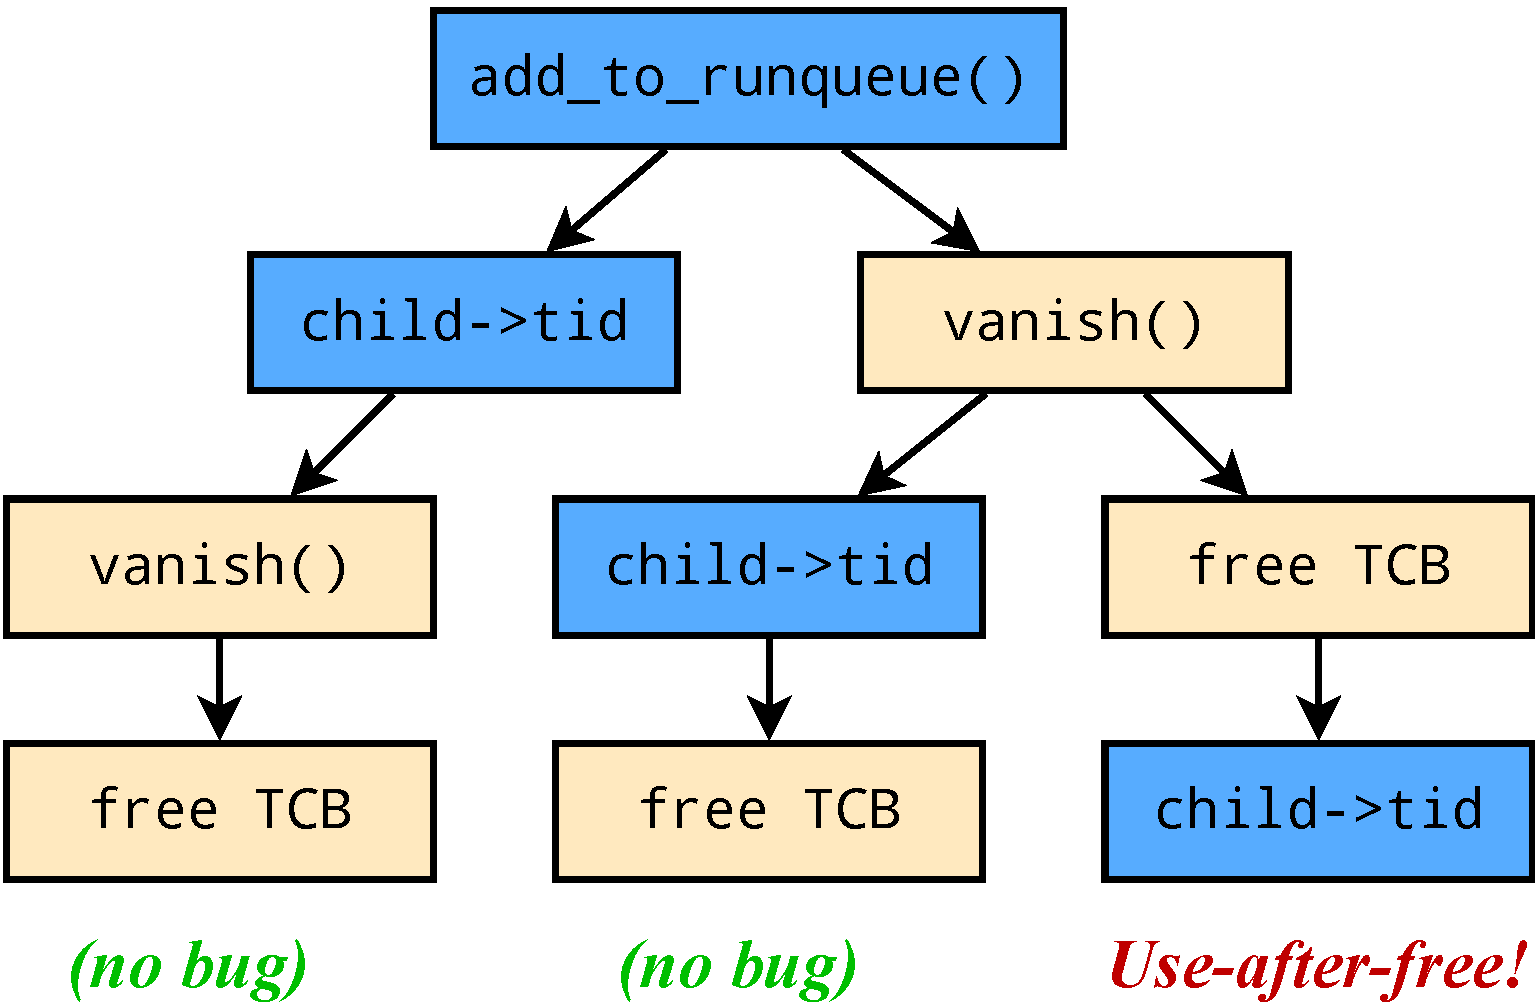
\includegraphics[width=0.42\textwidth]{threadfork/threadfork.pdf}
\caption{The state space of possible thread interleavings can be viewed as an {\em execution tree}.
Landslide uses timer interrupts to force different threads to run as it explores this tree.
If a kernel has concurrency errors, they will show up in some branches, but not others.
This tree shows the bug from Figure~\ref{fig:threadfork}, with operations from the parent thread shaded.
}
\label{fig:tree}
\end{figure}

%%%%%%%%%%%%%%%%%%%%%%%%%%%%%%%%%%%%%%%%%%%%%%%%%%%%%%%%%%%%%%%%%%%%%%%%%%%%%%%%
\subsection{Identifying Bugs}

Landslide has several checks that detect when a bug arises. It can identify kernel panics, use-after-free accesses (and other heap-related errors such as double-free and memory leaks), and
\shortversion{
deadlocks, and also includes a heuristic check for infinite loops and livelock.
}{
deadlocks.
Landslide can optionally also check heuristically for infinite loops and livelock. This is done by comparing the length of the current interleaving against previously-explored ones: if the current interleaving has been running disproportionately longer (by a large arbitrary constant factor), we assume the kernel is stuck.
We have not found this technique to erroneously report false positives, although it may fail to trigger when it ought to if too few previous interleavings have been tested to make a reliable comparison.
}

When Landslide identifies a bug, it outputs a
\shortversion
{{\em decision trace} (Figure~\ref{fig:trace}).}
{{\em decision trace}, an example of which is shown in Figure~\ref{fig:trace}.}
The trace reports what kind of bug was detected
\shortversion
{}
{(for uses-after-free, it also prints stack traces to show when the block was allocated and freed),}
and also reports each decision point in the current interleaving: which thread was running, a trace of its stack when it was switched away from, and the thread that Landslide caused to preempt it.
With this trace, the student can better understand the concurrent execution that exposed the bug.

Note that our use of the term ``race condition'' throughout this paper refers to concurrency errors in general, a category that includes data races, atomicity violations, and nondeterministic deadlocks.
In contrast with analyses that directly detect data races~\cite{tsan}, Landslide does not identify bugs at suspicious memory accesses, but rather detects failure conditions that can arise from many different types of errors.
\shortversion{}{
In general,
% with false-negative bug detection,
a kernel might contain a buggy behaviour that Landslide could overlook (i.e., a false negative). However (except in the case of heuristic infinite loop detection), when Landslide does identify a bug, the student can be sure that an error exists.
}

\newcommand\bug[1]{\hilight{red}{#1}}
\newcommand\decision[1]{\bfseries \hilight{olivegreen}{#1}}
\newcommand\stacktrace[1]{\hilight{darkcyan}{#1}}
\begin{figure}[t]
\small
\begin{lstlisting}
#\bfseries \bug{USE~AFTER~FREE:~read~from~0x15a8f0~at~IP~0x104209}#
#\bug{Block~0x15a8f0~was~allocated~by~thread~3~at~(...)}#
                   #\bug{and~freed~by~thread~4~at~(...)}#
Decision trace follows:
#\decision{1:  switched from thread 3 -> thread 4 at:}#
        0x105a10 in #\stacktrace{context\_switch}#,
        0x1041f4 in #\stacktrace{thread\_fork}#,
        0x10362b in #\stacktrace{thread\_fork\_wrapper}#
#\decision{2:  switched from thread 4 -> thread 3 at:}#
        0x105a10 in #\stacktrace{context\_switch}#,
        0x104681 in #\stacktrace{yield}#,
        0x104570 in #\stacktrace{exit}#,
        0x103708 in #\stacktrace{exit\_wrapper}#
#\decision{Current thread 3 at:}#
        0x104209 in #\stacktrace{thread\_fork}#,
        0x10362b in #\stacktrace{thread\_fork\_wrapper}#
Total decision points 24, total backtracks 5
\end{lstlisting}
\caption{Landslide outputs this trace for Figure~\ref{fig:threadfork}'s bug.}
\label{fig:trace}
\end{figure}

%%%%%%%%%%%%%%%%%%%%%%%%%%%%%%%%%%%%%%%%%%%%%%%%%%%%%%%%%%%%%%%%%%%%%%%%%%%%%%%%
\subsection{Instrumentation}
\label{sec:instrument}

Landslide's interface is comprised of two types of instrumentation which students must provide: {\em required annotations} and {\em configuring decision points}.

\subsubsection{Required annotations}
Users annotate their kernels to inform Landslide of certain important concurrency events during execution. We provide a set of annotation functions, named with the prefix \x{tell_landslide}, for this purpose. The annotations denote when a thread runs \x{fork}, \x{sleep}, or \x{exit}, when a thread is added to or removed from the runqueue, and when a thread becomes blocked on a mutex.
Figure~\ref{fig:annotation} shows annotated code corresponding to Figure~\ref{fig:threadfork}.

There is also a configuration file, \x{config.landslide}, in which the student must specify constant information such as the function names of the timer handler and context switcher, which threads exist when the kernel boots, and which user-space test program Landslide should invoke.
Finally, there are two short (nominally two-line) functions used within Landslide itself that the user must implement. These are predicates on the kernel's scheduler state, and express potentially nontrivial conditions: whether the current thread is runnable but not on the runqueue, and whether preemption is disabled while interrupts are on.

\newcommand\telllandslide[1]{\bfseries \color{violet}{#1}}
\begin{figure}[t]
\small
\begin{lstlisting}
void add_to_runqueue(thread_t *child) {
	#\telllandslide{tell\_landslide\_thread\_runnable(child->tid);}#
	// ...
}
int thread_fork() {
	thread_t *child = construct_new_thread();
	#\telllandslide{tell\_landslide\_forking(child->tid);}#
	add_to_runqueue(child);
	return child->tid;
}
\end{lstlisting}
\caption{Landslide requires the programmer to annotate important concurrency events\shortversion{.}{in their kernel.} \x{tell_landslide_thread_runnable()} indicates that a thread can henceforth be forced to run with timer interrupts, and \x{tell_landslide_forking()} announces a new thread's existence.}
\label{fig:annotation}
\end{figure}

\subsubsection{Configuring decision points}
\label{sec:decision}

Using only decision points that Landslide automatically identifies on voluntary reschedules will result in coarse-grained interleavings likely to overlook bugs.
We provide an extra annotation
for students to add more decision points for a finer-grained search, called
\x{tell_landslide_decide()}.
We recommend inserting it into concurrency primitives, such as at the start of \x{mutex_lock()} and at the end of \x{mutex_unlock()}.

\subsubsection{Focusing the search space}
\label{sec:focusing}

The strategy we describe above may cause Landslide to identify decision points in unrelated parts of the kernel, such as when accessing mutexes in unrelated and/or already-trusted system calls.
We provide interface options in \x{config.landslide} for the student to view currently identified decision points and to selectively eliminate them.
If a student were testing thread death and reaping, they might want decision points to appear in \x{wait} and \x{vanish} but not if unrelated virtual memory operations are also in progress.
Accordingly, they could write \x{within_function wait vanish} and \x{without_function} \x{destroy_address_space}.
The \x{within_function} directive requires that at least one of the specified functions shall be on the call stack when decision points are identified, and \x{without_function} requires the opposite.

% First, the student writes ``\x{DECISION_INFO_ONLY}'' to make Landslide run only one interleaving and then print all decision points instead of continuing to explore.
% In this file, students can write ``\x{within_function} \x{foo}'' to whitelist function \x{foo}, and ``\x{without_function} \x{bar}'' to blacklist function \x{bar}.
% In this file, students can use the ``\x{within_function}'' and ``\x{without_function}'' directives to require that given functions are or are not on the call stack when decision points are identified.
% make Landslide ignore any decision points that don't arise from the execution of specific functions.
% For example, if testing thread death and reaping, the student should write \x{within_function exit} and \x{within_function} \x{wait}, and also
% (assuming they don't care about the virtual memory operations associated with \x{exit})
% \x{without_function} \x{destroy_address_space}.

% Additionally, the student may configure Landslide's state space reduction to ignore certain memory locations.
% DPOR's analysis requires a memory independence relation between thread transitions; the more transitions are independent from each other, the more reduction can be achieved.
% Unfortunately, in the kernel environment, every thread switch will execute through a common path that modifies shared scheduler data structures.
% Unchecked, this would cause every transition to conflict with each other and result in no reduction in execution time from DPOR.
% Certain other shared memory conflicts also arise that are irrelevant to whichever system calls are being tested; for example, if testing for races in thread lifecycle routines, the user likely does not care about accesses to the frame allocator mutex.
%
% We provide an interface with which the user can configure Landslide to ignore such unrelated conflicts to more efficiently test components of the kernel they care about.
% In \x{config.landslide}, the user writes ``\x{ignore_sym}'' followed by the name of the global variable to ignore and its type size, and Landslide may then identify transitions as independent even if they conflict on that memory.

%%%%%%%%%%%%%%%%%%%%%%%%%%%%%%%%%%%%%%%%%%%%%%%%%%%%%%%%%%%%%%%%%%%%%%%%%%%%%%%%
\subsection{Limitations}

Landslide currently assumes that timer interrupts are the only nondeterministic events that influence a kernel's concurrent execution. While this prevents us from finding races related to external input such as disk or network I/O, Landslide is already able to find many types of complicated races by controlling timer-driven thread scheduling.
Landslide's model is also currently restricted to uniprocessor execution.
Supporting multiprocessor environments and device driver testing is left to future work.
% this used to say ", and production kernels"

In contrast with conventional stress testing, in which the test program exercises many system calls, Landslide works best with very small test cases.
Landslide's coverage results from exploring the different scheduling possibilities that arise from a short sequence of system calls.
If Landslide were used when running a stress test, the resulting state space would be too large to explore feasibly.
Hence, when working with students, we provided a suite of four test programs, each no longer than 10 lines of code, but carefully written to bring about system call interactions known to be troublesome.


\section{Outcomes}

\subsection{Teaching with Pebbles}

\framebox{Some text should go here!}

\subsection{Evaluating Landslide}

We evaluated Landslide in two ways: first, by instrumenting two kernels we were familiar with to measure time spent to find different races, and second, by meeting with students of 15-410 in the Spring 2012 semester, before they submitted their kernel for grading, to see if they could find bugs on their own with Landslide.

We instrumented one kernel written by an author in a previous year, and also one kernel the same author manually graded as a teaching assistant.
We configured Landslide to search for five complicated already-known race conditions.
In addition to finding all five races, Landslide also found a sixth previously unknown race in said author's own kernel.
Using decision points only on calls to \x{mutex_lock} and on voluntary reschedules, Landslide found each of the six bugs in 11 to 57 seconds, executing between 1 and 377 distinct interleavings for each.

In the user study of current students, we found that students spent on average 119 minutes (60 to 158) on the required instrumentation, and a further 36 minutes (10 to 60) refining Landslide's search.
Of the four groups who finished the required part, all four found previously unknown bugs with Landslide: two races and two deterministic errors.
These bugs manifested as infinite loops, a kernel panic, and a use-after-free.


% \section{Introduction}
% no \IEEEPARstart
% This demo file is intended to serve as a ``starter file''
% for IEEE conference papers produced under \LaTeX\ using
% IEEEtran.cls version 1.7 and later.
% 
% All manuscripts must be in English. These guidelines include complete descriptions of the fonts, spacing, and related information for producing your proceedings manuscripts. Please follow them and if you have any questions, direct them to the production editor in charge of your proceedings at Conference Publishing Services (CPS): Phone +1 (714) 821-8380 or Fax +1 (714) 761-1784.
% You must have at least 2 lines in the paragraph with the drop letter
% (should never be an issue)

% \subsection{Subsection Heading Here}
% Subsection text here.
% 
% 
% \subsubsection{Subsubsection Heading Here}
% Subsubsection text here.
% 
% \section{Type style and Fonts}
% Wherever Times is specified, Times Roman or Times New Roman may be used. If neither is available on your system, please use the font closest in appearance to Times. Avoid using bit-mapped fonts if possible. True-Type 1 or Open Type fonts are preferred. Please embed symbol fonts, as well, for math, etc.
% 

% An example of a floating figure using the graphicx package.
% Note that \label must occur AFTER (or within) \caption.
% For figures, \caption should occur after the \includegraphics.
% Note that IEEEtran v1.7 and later has special internal code that
% is designed to preserve the operation of \label within \caption
% even when the captionsoff option is in effect. However, because
% of issues like this, it may be the safest practice to put all your
% \label just after \caption rather than within \caption{}.
%
% Reminder: the "draftcls" or "draftclsnofoot", not "draft", class
% option should be used if it is desired that the figures are to be
% displayed while in draft mode.
%
%\begin{figure}[!t]
%\centering
%\includegraphics[width=2.5in]{myfigure}
% where an .eps filename suffix will be assumed under latex, 
% and a .pdf suffix will be assumed for pdflatex; or what has been declared
% via \DeclareGraphicsExtensions.
%\caption{Simulation Results}
%\label{fig_sim}
%\end{figure}

% Note that IEEE typically puts floats only at the top, even when this
% results in a large percentage of a column being occupied by floats.


% An example of a double column floating figure using two subfigures.
% (The subfig.sty package must be loaded for this to work.)
% The subfigure \label commands are set within each subfloat command, the
% \label for the overall figure must come after \caption.
% \hfil must be used as a separator to get equal spacing.
% The subfigure.sty package works much the same way, except \subfigure is
% used instead of \subfloat.
%
%\begin{figure*}[!t]
%\centerline{\subfloat[Case I]\includegraphics[width=2.5in]{subfigcase1}%
%\label{fig_first_case}}
%\hfil
%\subfloat[Case II]{\includegraphics[width=2.5in]{subfigcase2}%
%\label{fig_second_case}}}
%\caption{Simulation results}
%\label{fig_sim}
%\end{figure*}
%
% Note that often IEEE papers with subfigures do not employ subfigure
% captions (using the optional argument to \subfloat), but instead will
% reference/describe all of them (a), (b), etc., within the main caption.


% An example of a floating table. Note that, for IEEE style tables, the 
% \caption command should come BEFORE the table. Table text will default to
% \footnotesize as IEEE normally uses this smaller font for tables.
% The \label must come after \caption as always.
%
%\begin{table}[!t]
%% increase table row spacing, adjust to taste
%\renewcommand{\arraystretch}{1.3}
% if using array.sty, it might be a good idea to tweak the value of
% \extrarowheight as needed to properly center the text within the cells
%\caption{An Example of a Table}
%\label{table_example}
%\centering
%% Some packages, such as MDW tools, offer better commands for making tables
%% than the plain LaTeX2e tabular which is used here.
%\begin{tabular}{|c||c|}
%\hline
%One & Two\\
%\hline
%Three & Four\\
%\hline
%\end{tabular}
%\end{table}


% Note that IEEE does not put floats in the very first column - or typically
% anywhere on the first page for that matter. Also, in-text middle ("here")
% positioning is not used. Most IEEE journals/conferences use top floats
% exclusively. Note that, LaTeX2e, unlike IEEE journals/conferences, places
% footnotes above bottom floats. This can be corrected via the \fnbelowfloat
% command of the stfloats package.

\section{Future Work and Conclusion}
\label{sec:future}

we did stuff

\section*{Acknowledgments}

Many people have contributed to the development of
15-410 over the past decade.
Stephen Muckle, currently at Qualcomm, led
the switch to x86 projects running in Simics.
Nathaniel Wesley Filardo,
currently a Ph.D.\ candidate at Johns Hopkins,
increased the sanity of the build infrastructure,
designed the \x{swexn()} system call, and helped critique this paper.
The current reference kernel is named ``pathos''
and was written by Michael J. Sullivan,
currently a CMU CS Ph.D.\ candidate,
and Elly Fong-Jones, currently at Google.
The SMP infrastructure code was contributed by
Ryan Pearl, currently at Mozilla.
Joshua Wise, currently at NVIDIA,
proposed and led several kernel-extension projects,
including the hypervisor project.
Over the past decade the course has benefitted
greatly from free educational Simics licenses,
donated initially by Virtutech and recently by
Wind River.
Code-size numbers were generated using David A.\ Wheeler's
``SLOCCount.''




% trigger a \newpage just before the given reference
% number - used to balance the columns on the last page
% adjust value as needed - may need to be readjusted if
% the document is modified later
%\IEEEtriggeratref{8}
% The "triggered" command can be changed if desired:
%\IEEEtriggercmd{\enlargethispage{-5in}}

% references section

\bibliographystyle{IEEEtran}
\bibliography{IEEEabrv,citations}





% that's all folks
\end{document}


